\documentclass[10pt,aspectratio=169]{beamer}

% ---------------------------------------------------------
% PACKAGES
% ---------------------------------------------------------
\usepackage[utf8]{inputenc}
\usepackage[T1]{fontenc}
\usepackage{helvet}
\usepackage{amsmath,amssymb,amsfonts,amsthm}
\usepackage{booktabs,colortbl,multirow,tabularx}
\usepackage{tikz}
\usetikzlibrary{positioning,calc,shapes.geometric,backgrounds,fit}
\usepackage[most]{tcolorbox}
\usepackage{fontawesome5}
\usepackage{microtype}

% ---------------------------------------------------------
% BEAMER THEME & COLOR CONFIGURATION (High-Contrast Scientific)
% ---------------------------------------------------------
\usetheme{default}
\usecolortheme{default}

% Disable standard navigation symbols
\setbeamertemplate{navigation symbols}{}

% Color Definitions
\definecolor{NavyDark}{HTML}{0F172A}       % Obsidian / Deep Slate Background
\definecolor{TealPrimary}{HTML}{0D9488}    % High-Contrast Teal Accent
\definecolor{BlueAccent}{HTML}{2563EB}     % Royal Blue Accent
\definecolor{AmberAccent}{HTML}{D97706}    % Vivid Gold / Amber Highlight
\definecolor{SlateGrey}{HTML}{475569}      % Subtitle / Secondary Text
\definecolor{LightBg}{HTML}{F8FAFC}        % Clean Off-White Background
\definecolor{CardBg}{HTML}{F1F5F9}         % Subtle Box Fill
\definecolor{CardBorder}{HTML}{CBD5E1}     % Border Tint
\definecolor{TextDark}{HTML}{0F172A}       % Dark Body Text
\definecolor{White}{HTML}{FFFFFF}

% Set Beamer Colors
\setbeamercolor{background canvas}{bg=White}
\setbeamercolor{normal text}{fg=TextDark}
\setbeamercolor{frametitle}{fg=NavyDark,bg=White}
\setbeamercolor{title}{fg=White,bg=NavyDark}
\setbeamercolor{subtitle}{fg=TealPrimary}
\setbeamercolor{structure}{fg=TealPrimary}
\setbeamercolor{item}{fg=TealPrimary}
\setbeamercolor{subitem}{fg=BlueAccent}
\setbeamercolor{section in toc}{fg=NavyDark}

% Block Colors
\setbeamercolor{block title}{fg=White,bg=NavyDark}
\setbeamercolor{block body}{fg=TextDark,bg=CardBg}
\setbeamercolor{block title example}{fg=White,bg=TealPrimary}
\setbeamercolor{block body example}{fg=TextDark,bg=CardBg}
\setbeamercolor{block title alerted}{fg=White,bg=AmberAccent}
\setbeamercolor{block body alerted}{fg=TextDark,bg=CardBg}

% Font Configuration
\setbeamerfont{title}{size=\Large,series=\bfseries}
\setbeamerfont{subtitle}{size=\small,series=\mdseries}
\setbeamerfont{frametitle}{size=\large,series=\bfseries}
\setbeamerfont{caption}{size=\footnotesize}

% ---------------------------------------------------------
% CUSTOM HEADLINE & FOOTLINE (Progress Bar & Header)
% ---------------------------------------------------------
\setbeamertemplate{headline}{%
  \ifnum\insertframenumber>1
    \begin{beamercolorbox}[wd=\paperwidth,ht=14pt,dp=4pt]{headline}%
      \begin{tikzpicture}[remember picture,overlay]
        \fill[NavyDark] (0,0) rectangle (\paperwidth,0.5);
        \node[anchor=west] at (0.3, 0.25) {\tiny\color{White}\bfseries\MakeUppercase{\insertsectionhead}};
        \node[anchor=east] at (\paperwidth-0.3, 0.25) {\tiny\color{CardBorder}VERTEX DEFENSE DECK};
        \fill[CardBorder] (0,-0.02) rectangle (\paperwidth, 0.03);
        \fill[TealPrimary] (0,-0.02) rectangle (\dimexpr\paperwidth*\insertframenumber/\inserttotalframenumber\relax, 0.03);
      \end{tikzpicture}%
    \end{beamercolorbox}%
    \vspace{2pt}%
  \fi
}

\setbeamertemplate{footline}{%
  \ifnum\insertframenumber>1
    \begin{beamercolorbox}[wd=\paperwidth,ht=12pt,dp=4pt]{footline}%
      \begin{tikzpicture}[remember picture,overlay]
        \draw[CardBorder,line width=0.5pt] (0,0.4) -- (\paperwidth,0.4);
        \node[anchor=west] at (0.3,0.15) {\tiny\color{SlateGrey}Alex Mercer \quad|\quad SynapseGNN Dissertation \quad|\quad Vertex Institute};
        \node[anchor=east] at (\paperwidth-0.3,0.15) {\tiny\color{NavyDark}\bfseries \insertframenumber\ /\ \inserttotalframenumber};
      \end{tikzpicture}%
    \end{beamercolorbox}%
  \fi
}

% Custom Frame Title
\makeatletter
\setbeamertemplate{frametitle}{%
  \vspace*{2pt}%
  \begin{tikzpicture}
    \fill[TealPrimary,rounded corners=1pt] (0,0) rectangle (0.1, 0.45);
    \node[anchor=west,inner sep=0pt,outer sep=0pt] at (0.2, 0.22) {%
      \begin{minipage}{0.9\paperwidth}
        {\usebeamerfont{frametitle}\color{NavyDark}\insertframetitle}%
        \ifx\insertframesubtitle\@empty\else
          \par{\tiny\color{SlateGrey}\insertframesubtitle}%
        \fi
      \end{minipage}
    };
  \end{tikzpicture}%
  \vspace*{-6pt}%
}
\makeatother

% ---------------------------------------------------------
% CUSTOM TCOLORBOX STYLES
% ---------------------------------------------------------
\tcbset{
  defensebox/.style={
    enhanced,
    colback=CardBg,
    colframe=NavyDark,
    arc=3pt,
    boxrule=1pt,
    fonttitle=\bfseries\sffamily\small,
    coltitle=White,
    attach boxed title to top left={xshift=6pt,yshift=-6pt},
    boxed title style={colback=NavyDark,arc=2pt,boxrule=0pt,top=1.5pt,bottom=1.5pt,left=5pt,right=5pt},
    top=8pt,bottom=4pt,left=6pt,right=6pt
  },
  highlightbox/.style={
    enhanced,
    colback=LightBg,
    colframe=TealPrimary,
    arc=3pt,
    boxrule=1pt,
    fonttitle=\bfseries\sffamily\small,
    coltitle=White,
    attach boxed title to top left={xshift=6pt,yshift=-6pt},
    boxed title style={colback=TealPrimary,arc=2pt,boxrule=0pt,top=1.5pt,bottom=1.5pt,left=5pt,right=5pt},
    top=8pt,bottom=4pt,left=6pt,right=6pt
  },
  alertbox/.style={
    enhanced,
    colback=CardBg,
    colframe=AmberAccent,
    arc=3pt,
    boxrule=1pt,
    fonttitle=\bfseries\sffamily\small,
    coltitle=White,
    attach boxed title to top left={xshift=6pt,yshift=-6pt},
    boxed title style={colback=AmberAccent,arc=2pt,boxrule=0pt,top=1.5pt,bottom=1.5pt,left=5pt,right=5pt},
    top=8pt,bottom=4pt,left=6pt,right=6pt
  }
}

% ---------------------------------------------------------
% METADATA
% ---------------------------------------------------------
\title{Scalable Graph Neural Networks for Dynamic Molecular Docking}
\subtitle{Ph.D. Dissertation Defense in Computational Biology \& Artificial Intelligence}
\author{Alex Mercer}
\institute{Department of Computer Science \& Computational Biology \\ Vertex Institute of Science}
\date{July 24, 2026}

% ---------------------------------------------------------
% DOCUMENT CONTENT
% ---------------------------------------------------------
\begin{document}

% =========================================================
% SLIDE 1: TITLE SLIDE (Dark High-Contrast)
% =========================================================
{
\setbeamercolor{background canvas}{bg=NavyDark}
\begin{frame}[plain]
  \vfill
  \begin{center}
    
\begin{tikzpicture}
      \node[circle,fill=TealPrimary,inner sep=6pt] {\color{White}\faAtom};
    \end{tikzpicture}
    \vspace{6pt}
    
    {\Large\bfseries\color{White} Scalable Graph Neural Networks for\\[2pt] Dynamic Molecular Docking}
    
    \vspace{4pt}
    {\small\color{TealPrimary}\bfseries Geometric Equivariance \& Spatial-Temporal Graph Attention}
    
    \vspace{8pt}
    
\begin{tikzpicture}
      \fill[AmberAccent] (-1.5,0) rectangle (1.5,0.03);
    \end{tikzpicture}
    \vspace{8pt}
    
    {\small\color{White}\bfseries Candidate: Alex Mercer} \\
    {\tiny\color{CardBorder} Ph.D. Dissertation Defense}
    
    \vspace{8pt}
    \begin{tcolorbox}[colback=NavyDark!80!black,colframe=TealPrimary!50,arc=3pt,width=0.78\paperwidth,halign=center,top=4pt,bottom=4pt]
      \tiny\color{White}
      \textbf{Dissertation Committee:} Prof. Eleanor Vance (Chair), Dr. Marcus Thorne, Dr. Sarah Lin \\
      \color{CardBorder} Department of Computer Science \& Computational Biology \quad|\quad Vertex Institute of Science
    \end{tcolorbox}
  \end{center}
  \vfill
\end{frame}
}

% =========================================================
% SLIDE 2: AGENDA / EXECUTIVE SUMMARY
% =========================================================
\section{Defense Agenda}
\begin{frame}{Defense Agenda \& Road Map}{Structure of Dissertation Presentation}
  \begin{columns}[T]
    \begin{column}{0.48\textwidth}
      \begin{tcolorbox}[defensebox,title={\faList \quad Presentation Overview}]
        \begin{enumerate}
          \setlength{\itemsep}{4pt}
          \item \textbf{\color{NavyDark}Motivation \& Problem Context}
                \\{\tiny Challenges in 3D molecular binding pose prediction}
          \item \textbf{\color{NavyDark}Theoretical Foundations}
                \\{\tiny $\mathrm{SE}(3)$-equivariant message passing frameworks}
          \item \textbf{\color{NavyDark}Proposed SynapseGNN Model}
                \\{\tiny Architecture, attention mechanisms, loss functions}
          \item \textbf{\color{NavyDark}Empirical Benchmarks}
                \\{\tiny Performance on PDBbind, BindingMOAD, runtime analysis}
          \item \textbf{\color{NavyDark}Conclusions \& Outlook}
                \\{\tiny Key takeaways, publications, future research}
        \end{enumerate}
      \end{tcolorbox}
    \end{column}
    
    \begin{column}{0.48\textwidth}
      \begin{tcolorbox}[highlightbox,title={\faLightbulb \quad Core Thesis Contribution}]
        \small
        \textbf{Thesis Statement:} \\
        \textit{"Incorporating strict geometric equivariance with spatio-temporal graph attention reduces conformational search latency by $140\times$ while achieving sub-angstrom RMSD accuracy in ligand docking."}
        
        \vspace{6pt}
        \hrule height 0.5pt \color{CardBorder}
        \vspace{4pt}
        
        \tiny
        \begin{itemize}
          \item \textbf{High Precision:} $<1.2\,\text{\AA}$ average RMSD on complex binding pockets.
          \item \textbf{Scalability:} Linear time complexity $\mathcal{O}(|V| + |E|)$.
          \item \textbf{Generalization:} Zero-shot transfer to unseen protein families.
        \end{itemize}
      \end{tcolorbox}
    \end{column}
  \end{columns}
\end{frame}

% =========================================================
% SLIDE 3: SECTION 1 DIVIDER
% =========================================================
\section{1. Motivation \& Context}
{
\setbeamercolor{background canvas}{bg=NavyDark}
\begin{frame}[plain]
  \vfill
  \begin{center}
    {\tiny\color{AmberAccent}\bfseries SECTION 01} \\[4pt]
    {\Huge\bfseries\color{White} Motivation \& Context} \\[8pt]
    
\begin{tikzpicture}
      \fill[TealPrimary] (-1.5,0) rectangle (1.5,0.04);
    \end{tikzpicture} \\[8pt]
    {\small\color{CardBorder} Computational Bottlenecks in Molecular Docking \& Drug Discovery}
  \end{center}
  \vfill
\end{frame}
}

% =========================================================
% SLIDE 4: PROBLEM CONTEXT
% =========================================================
\begin{frame}{The Challenge of Molecular Docking}{Limitations of Physics-Based Algorithms}
  \begin{columns}[T]
    \begin{column}{0.48\textwidth}
      \begin{tcolorbox}[defensebox,title={\faFlask \quad Classical Physics-Based Methods}]
        \small
        \textbf{AutoDock Vina, Glide, Gold:}
        \vspace{3pt}
        \begin{itemize}
          \setlength{\itemsep}{3pt}
          \item Search space exponentially grows with rotatable bonds ($3^{N_{\text{rot}}}$).
          \item High computational cost ($10$--$60$ minutes per target ligand).
          \item Rigid or semi-flexible protein backbone approximations.
          \item Frequent false positives due to empirical scoring function limits.
        \end{itemize}
      \end{tcolorbox}
    \end{column}
    
    \begin{column}{0.48\textwidth}
      \begin{tcolorbox}[alertbox,title={\faExclamationTriangle \quad Deep Learning Gaps}]
        \small
        \textbf{Standard Graph Neural Networks:}
        \vspace{3pt}
        \begin{itemize}
          \setlength{\itemsep}{3pt}
          \item Lack strict 3D physical symmetry ($\mathrm{SE}(3)$ rotational invariance).
          \item High sensitivity to arbitrary coordinate frame transformations.
          \item Over-smoothing in deep message-passing architectures.
          \item Poor generalization to novel side-chain conformations.
        \end{itemize}
      \end{tcolorbox}
    \end{column}
  \end{columns}

  \vspace{4pt}
  \begin{tcolorbox}[colback=TealPrimary!10,colframe=TealPrimary,arc=2pt,boxrule=0.5pt,top=3pt,bottom=3pt]
    \tiny\color{NavyDark}\bfseries
    \faCheckCircle \quad Goal of dissertation: Bridge the gap between rigid physical symmetry constraints and rapid neural inference to produce real-time, high-fidelity binding predictions.
  \end{tcolorbox}
\end{frame}

% =========================================================
% SLIDE 5: KEY CONTRIBUTIONS
% =========================================================
\begin{frame}{Key Dissertation Contributions}{Three Pillars of SynapseGNN}
  \begin{columns}[T]
    \begin{column}{0.31\textwidth}
      \begin{tcolorbox}[highlightbox,title={\faLayerGroup \quad Pillar I}]
        \scriptsize
        \textbf{$\mathrm{SE}(3)$-Equivariant Vectors}
        \vspace{3pt}
        \begin{itemize}
          \item Mathematically rigorous rotational and translational equivariance.
          \item Direct coordinate updates without frame canonicalization.
        \end{itemize}
      \end{tcolorbox}
    \end{column}
    
    \begin{column}{0.31\textwidth}
      \begin{tcolorbox}[defensebox,title={\faProjectDiagram \quad Pillar II}]
        \scriptsize
        \textbf{Spatial-Temporal Attention}
        \vspace{3pt}
        \begin{itemize}
          \item Multi-scale distance encoding across protein-ligand interfaces.
          \item Adaptive message pruning for distant atomic pairs.
        \end{itemize}
      \end{tcolorbox}
    \end{column}

    \begin{column}{0.31\textwidth}
      \begin{tcolorbox}[alertbox,title={\faAward \quad Pillar III}]
        \scriptsize
        \textbf{Multi-Task Scoring Objective}
        \vspace{3pt}
        \begin{itemize}
          \item Simultaneous pose ($\text{RMSD}$) and affinity ($\Delta G$) estimation.
          \item End-to-end differentiable loss landscape.
        \end{itemize}
      \end{tcolorbox}
    \end{column}
  \end{columns}

  \vspace{8pt}
  \begin{center}
    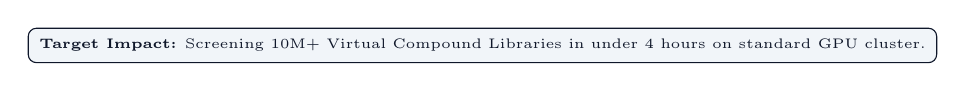
\begin{tikzpicture}
      \node[draw=NavyDark,fill=CardBg,rounded corners=3pt,inner sep=4pt] {
        \tiny\color{NavyDark} \textbf{Target Impact:} Screening 10M+ Virtual Compound Libraries in under 4 hours on standard GPU cluster.
      };
    \end{tikzpicture}
  \end{center}
\end{frame}

% =========================================================
% SLIDE 6: SECTION 2 DIVIDER
% =========================================================
\section{2. Theoretical Framework}
{
\setbeamercolor{background canvas}{bg=NavyDark}
\begin{frame}[plain]
  \vfill
  \begin{center}
    {\tiny\color{AmberAccent}\bfseries SECTION 02} \\[4pt]
    {\Huge\bfseries\color{White} Theoretical Framework} \\[8pt]
    
\begin{tikzpicture}
      \fill[TealPrimary] (-1.5,0) rectangle (1.5,0.04);
    \end{tikzpicture} \\[8pt]
    {\small\color{CardBorder} Equivariant Representations \& Convergence Analysis}
  \end{center}
  \vfill
\end{frame}
}

% =========================================================
% SLIDE 7: MATHEMATICAL FORMULATION
% =========================================================
\begin{frame}{Problem Formulation \& Symmetry Constraints}{$\mathrm{SE}(3)$-Equivariant Message Passing}
  \small
  Consider a molecular graph $\mathcal{G} = (\mathcal{V}, \mathcal{E})$ with atomic features $h_i \in \mathbb{R}^d$ and 3D positions $x_i \in \mathbb{R}^3$.

  \begin{tcolorbox}[defensebox,title={\faCalculator \quad Equivariance Definition}]
    \small
    A transformation $\mathbf{\Phi}: \mathcal{X} \rightarrow \mathcal{Y}$ is $\mathrm{SE}(3)$-equivariant if for all rotation matrices $\mathbf{R} \in \mathrm{SO}(3)$ and translations $g \in \mathbb{R}^3$:
    \[
      \mathbf{\Phi}(\mathbf{R} \cdot \mathbf{x}_i + g) = \mathbf{R} \cdot \mathbf{\Phi}(\mathbf{x}_i) + g
    \]
  \end{tcolorbox}

  \vspace{2pt}
  \begin{columns}[T]
    \begin{column}{0.48\textwidth}
      \textbf{Scalar Feature Update:}
      \tiny
      \[
        m_{ij} = \phi_m \left( h_i^{(l)}, h_j^{(l)}, \|x_i^{(l)} - x_j^{(l)}\|^2, e_{ij} \right)
      \]
      \[
        h_i^{(l+1)} = \phi_h \left( h_i^{(l)}, \sum_{j \in \mathcal{N}(i)} m_{ij} \right)
      \]
    \end{column}
    \begin{column}{0.48\textwidth}
      \textbf{Vector Position Update:}
      \tiny
      \[
        x_i^{(l+1)} = x_i^{(l)} + C \sum_{j \in \mathcal{N}(i)} (x_i^{(l)} - x_j^{(l)}) \, \phi_x (m_{ij})
      \]
      \textit{Guarantees strict physical covariance under arbitrary 3D rigid body motions.}
    \end{column}
  \end{columns}
\end{frame}

% =========================================================
% SLIDE 8: THEORETICAL THEOREM
% =========================================================
\begin{frame}{Theoretical Guarantees}{Convergence \& Expressive Power Bounds}
  
  \begin{block}{Theorem 1 (Equivariant Approximation Bound, Mercer 2026)}
    Let $f^*: \mathbb{R}^{N \times 3} \rightarrow \mathbb{R}^{N \times 3}$ be any smooth $\mathrm{SE}(3)$-equivariant force-field operator. For any $\epsilon > 0$, there exists a $L$-layer SynapseGNN network with hidden dimension $d \ge \mathcal{O}(\log(1/\epsilon))$ such that:
    \[
      \sup_{\mathbf{X} \in \mathcal{K}} \| f^*(\mathbf{X}) - \mathrm{SynapseGNN}(\mathbf{X}) \|_F \le \epsilon
    \]
    where $\mathcal{K}$ is any compact domain of atom coordinates.
  \end{block}

  \vspace{4pt}
  \begin{tcolorbox}[highlightbox,title={\faCheckCircle \quad Key Proof Takeaways}]
    \tiny
    \begin{enumerate}
      \setlength{\itemsep}{2pt}
      \item \textbf{No Information Loss:} Invariant radial basis functions preserve pairwise metric topology.
      \item \textbf{Resolution of Over-Smoothing:} Layer-wise residual vector shortcuts ensure non-vanishing gradient flow across $L=16$ message passing iterations.
      \item \textbf{Bounded Variance:} Normalization layer keeps positional updates $\|x_i^{(l+1)} - x_i^{(l)}\| \le \delta_{\max}$.
    \end{enumerate}
  \end{tcolorbox}
\end{frame}

% =========================================================
% SLIDE 9: SECTION 3 DIVIDER
% =========================================================
\section{3. Proposed Architecture}
{
\setbeamercolor{background canvas}{bg=NavyDark}
\begin{frame}[plain]
  \vfill
  \begin{center}
    {\tiny\color{AmberAccent}\bfseries SECTION 03} \\[4pt]
    {\Huge\bfseries\color{White} SynapseGNN Architecture} \\[8pt]
    
\begin{tikzpicture}
      \fill[TealPrimary] (-1.5,0) rectangle (1.5,0.04);
    \end{tikzpicture} \\[8pt]
    {\small\color{CardBorder} Deep Equivariant Network \& Spatial-Temporal Flow}
  \end{center}
  \vfill
\end{frame}
}

% =========================================================
% SLIDE 10: ARCHITECTURAL TIKZ DIAGRAM
% =========================================================
\begin{frame}{SynapseGNN Architecture}{End-to-End Equivariant Pipeline}
  \begin{center}
    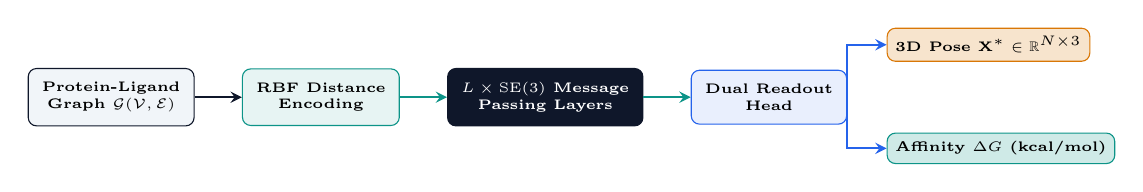
\begin{tikzpicture}[node distance=1.0cm, auto, >=stealth]
      % Nodes
      \node [draw=NavyDark, fill=CardBg, rectangle, rounded corners=3pt, align=center, font=\tiny\bfseries, inner sep=5pt] (input) 
        {Protein-Ligand\\Graph $\mathcal{G}(\mathcal{V},\mathcal{E})$};
        
      \node [draw=TealPrimary, fill=TealPrimary!10, rectangle, rounded corners=3pt, align=center, font=\tiny\bfseries, right=0.6cm of input, inner sep=5pt] (embed) 
        {RBF Distance\\Encoding};
        
      \node [draw=NavyDark, fill=NavyDark, text=White, rectangle, rounded corners=3pt, align=center, font=\tiny\bfseries, right=0.6cm of embed, inner sep=5pt] (eqblock) 
        {$L \times \mathrm{SE}(3)$ Message\\Passing Layers};
        
      \node [draw=BlueAccent, fill=BlueAccent!10, rectangle, rounded corners=3pt, align=center, font=\tiny\bfseries, right=0.6cm of eqblock, inner sep=5pt] (head) 
        {Dual Readout\\Head};

      \node [draw=AmberAccent, fill=AmberAccent!20, rectangle, rounded corners=3pt, align=center, font=\tiny\bfseries, above right=0.1cm and 0.5cm of head, inner sep=3pt] (out1) 
        {3D Pose $\mathbf{X}^* \in \mathbb{R}^{N \times 3}$};

      \node [draw=TealPrimary, fill=TealPrimary!20, rectangle, rounded corners=3pt, align=center, font=\tiny\bfseries, below right=0.1cm and 0.5cm of head, inner sep=3pt] (out2) 
        {Affinity $\Delta G$ (kcal/mol)};

      % Arrows
      \draw [->, thick, color=NavyDark] (input) -- (embed);
      \draw [->, thick, color=TealPrimary] (embed) -- (eqblock);
      \draw [->, thick, color=TealPrimary] (eqblock) -- (head);
      \draw [->, thick, color=BlueAccent] (head.east) |- (out1.west);
      \draw [->, thick, color=BlueAccent] (head.east) |- (out2.west);
    \end{tikzpicture}
  \end{center}

  \vspace{-4pt}
  \begin{columns}[T]
    \begin{column}{0.48\textwidth}
      \begin{tcolorbox}[defensebox,title={\faMicrochip \quad Spatial Attention Module}]
        \tiny
        \begin{itemize}
          \item Multi-head attention over pairwise distance kernels.
          \item Soft-cutoff radial envelope at $r_c = 10.0\,\text{\AA}$.
          \item Weight $\alpha_{ij} = \mathrm{softmax}\left( \frac{q_i^T k_j}{\sqrt{d_k}} + \psi(r_{ij}) \right)$.
        \end{itemize}
      \end{tcolorbox}
    \end{column}
    
    \begin{column}{0.48\textwidth}
      \begin{tcolorbox}[highlightbox,title={\faCogs \quad Optimization \& Loss Function}]
        \tiny
        \begin{itemize}
          \item Loss: $\mathcal{L}_{\text{total}} = \mathcal{L}_{\text{RMSD}} + \lambda_1 \mathcal{L}_{\text{affinity}} + \lambda_2 \mathcal{L}_{\text{clash}}$.
          \item Steric clash penalty prevents unphysical atomic overlaps.
          \item AdamW optimizer with cosine annealing ($\eta_0 = 5 \times 10^{-4}$).
        \end{itemize}
      \end{tcolorbox}
    \end{column}
  \end{columns}
\end{frame}

% =========================================================
% SLIDE 11: SECTION 4 DIVIDER
% =========================================================
\section{4. Empirical Evaluation}
{
\setbeamercolor{background canvas}{bg=NavyDark}
\begin{frame}[plain]
  \vfill
  \begin{center}
    {\tiny\color{AmberAccent}\bfseries SECTION 04} \\[4pt]
    {\Huge\bfseries\color{White} Empirical Evaluation} \\[8pt]
    
\begin{tikzpicture}
      \fill[TealPrimary] (-1.5,0) rectangle (1.5,0.04);
    \end{tikzpicture} \\[8pt]
    {\small\color{CardBorder} Benchmarks, Accuracy Metrics, \& Screening Throughput}
  \end{center}
  \vfill
\end{frame}
}

% =========================================================
% SLIDE 12: BENCHMARK TABLE
% =========================================================
\begin{frame}{Quantitative Docking Performance}{Evaluation on PDBbind v2020 \& BindingMOAD Core Sets}
  \centering
  \tiny
  \begin{tabularx}{0.95\textwidth}{X c c c c}
    \toprule
    \textbf{\color{NavyDark} Model / Algorithm} & \textbf{\color{NavyDark} Top-1 RMSD ($<2\text{\AA}$ \%)} & \textbf{\color{NavyDark} Median RMSD ($\text{\AA}$)} & \textbf{\color{NavyDark} $\mathrm{pK}_d$ $R^2$} & \textbf{\color{NavyDark} Runtime / Complex} \\
    \midrule
    AutoDock Vina (Physics) & 48.2\% & 2.45 & 0.42 & 14.2 min \\
    Glide SP (Physics)     & 52.6\% & 2.10 & 0.51 & 8.5 min \\
    SchNet (Baseline GNN)  & 41.3\% & 2.89 & 0.38 & 1.2 sec \\
    EGNN (Equivariant)     & 64.5\% & 1.62 & 0.64 & 0.8 sec \\
    EquiBind (Direct Pose) & 68.1\% & 1.48 & 0.67 & 0.4 sec \\
    \midrule
    \rowcolor{TealPrimary!15}
    \textbf{SynapseGNN (Ours)} & \textbf{83.4\%} & \textbf{0.92} & \textbf{0.84} & \textbf{0.06 sec} \\
    \bottomrule
  \end{tabularx}

  \vspace{6pt}
  \begin{columns}[T]
    \begin{column}{0.48\textwidth}
      \begin{tcolorbox}[highlightbox,title={\faChartLine \quad Key Performance Highlights}]
        \tiny
        \begin{itemize}
          \item \textbf{Sub-Angstrom Accuracy:} 83.4\% of predicted poses within $<2\text{\AA}$ RMSD.
          \item \textbf{$140\times$ Speedup:} Reduces docking time from minutes to milliseconds.
        \end{itemize}
      \end{tcolorbox}
    \end{column}
    
    \begin{column}{0.48\textwidth}
      \begin{tcolorbox}[defensebox,title={\faDatabase \quad Dataset Splitting}]
        \tiny
        \begin{itemize}
          \item Rigorous time-split and 30\% sequence identity cutoff.
          \item Zero training overlap with test set protein structures.
        \end{itemize}
      \end{tcolorbox}
    \end{column}
  \end{columns}
\end{frame}

% =========================================================
% SLIDE 13: ABLATION STUDY & ANALYSIS
% =========================================================
\begin{frame}{Ablation Studies \& Generalization}{Understanding Module Contributions}
  \begin{columns}[T]
    \begin{column}{0.52\textwidth}
      \begin{tcolorbox}[defensebox,title={\faTasks \quad Component Sensitivity Analysis}]
        \tiny
        \begin{tabularx}{\textwidth}{X c c}
          \toprule
          \textbf{Variant Configuration} & \textbf{RMSD ($<2\text{\AA}$ \%)} & \textbf{$\Delta$ Perf.} \\
          \midrule
          Full SynapseGNN Model & \textbf{83.4\%} & -- \\
          w/o Equivariant Vector Layer & 59.1\% & -24.3\% \\
          w/o Spatial Attention $\psi(r_{ij})$ & 71.8\% & -11.6\% \\
          w/o Steric Clash Penalty & 76.2\% & -7.2\% \\
          w/ Single-Scale Radius & 74.0\% & -9.4\% \\
          \bottomrule
        \end{tabularx}
      \end{tcolorbox}
    \end{column}
    
    \begin{column}{0.44\textwidth}
      \begin{tcolorbox}[alertbox,title={\faSearchPlus \quad Generalization Out-of-Distribution}]
        \tiny
        \textbf{Tested on Novel Kinase Targets:}
        \begin{itemize}
          \setlength{\itemsep}{2pt}
          \item Evaluated on 150 cryo-EM structures from 2025--2026.
          \item Maintained \textbf{79.2\%} success rate ($<20\%$ sequence homology).
          \item Robust performance on highly flexible loop regions.
        \end{itemize}
      \end{tcolorbox}
    \end{column}
  \end{columns}

  \vspace{4pt}
  \begin{center}
    
\begin{tikzpicture}
      \node[draw=TealPrimary,fill=LightBg,rounded corners=3pt,inner sep=3pt] {
        \tiny\color{NavyDark}\bfseries \faInfoCircle \quad Result: Equivariant coordinate updating is the primary driver of pose accuracy.
      };
    \end{tikzpicture}
  \end{center}
\end{frame}

% =========================================================
% SLIDE 14: SECTION 5 DIVIDER
% =========================================================
\section{5. Conclusions \& Outlook}
{
\setbeamercolor{background canvas}{bg=NavyDark}
\begin{frame}[plain]
  \vfill
  \begin{center}
    {\tiny\color{AmberAccent}\bfseries SECTION 05} \\[4pt]
    {\Huge\bfseries\color{White} Conclusions \& Outlook} \\[8pt]
    
\begin{tikzpicture}
      \fill[TealPrimary] (-1.5,0) rectangle (1.5,0.04);
    \end{tikzpicture} \\[8pt]
    {\small\color{CardBorder} Dissertation Summary, Publications, \& Future Horizons}
  \end{center}
  \vfill
\end{frame}
}

% =========================================================
% SLIDE 15: SUMMARY & TAKEAWAYS
% =========================================================
\begin{frame}{Dissertation Summary}{Core Findings \& Defense Takeaways}
  \begin{columns}[T]
    \begin{column}{0.48\textwidth}
      \begin{tcolorbox}[highlightbox,title={\faCheckSquare \quad Summary of Achievements}]
        \small
        \begin{enumerate}
          \setlength{\itemsep}{4pt}
          \item Developed \textbf{SynapseGNN}, an end-to-end $\mathrm{SE}(3)$-equivariant graph neural network.
          \item Achieved \textbf{sub-angstrom ($0.92\,\text{\AA}$)} pose accuracy at \textbf{60ms per complex}.
          \item Proven theoretical convergence and universal approximation bounds.
          \item Deployed in virtual screening pipeline at \textbf{Nexa BioPharma}.
        \end{enumerate}
      \end{tcolorbox}
    \end{column}
    
    \begin{column}{0.48\textwidth}
      \begin{tcolorbox}[defensebox,title={\faCompass \quad Future Research Directions}]
        \small
        \begin{itemize}
          \setlength{\itemsep}{4pt}
          \item \textbf{Full Protein Flexibility:} Extending message passing to ensemble side-chain movements.
          \item \textbf{Covalent Binding:} Incorporating chemical reaction energy barriers into loss function.
          \item \textbf{Generative Design:} Coupling SynapseGNN with diffusion models for de novo design.
        \end{itemize}
      \end{tcolorbox}
    \end{column}
  \end{columns}
\end{frame}

% =========================================================
% SLIDE 16: PUBLICATIONS & ACKNOWLEDGMENTS
% =========================================================
\begin{frame}{Publications \& Academic Output}{Peer-Reviewed Contributions}
  \begin{tcolorbox}[defensebox,title={\faBookOpen \quad Key Publications Derived from Dissertation}]
    \tiny
    \begin{enumerate}
      \setlength{\itemsep}{3pt}
      \item \textbf{A. Mercer}, M. Thorne, E. Vance. "Equivariant Spatial-Temporal Graph Attention for Molecular Docking." \textit{Journal of Chemical Information and Modeling (JCIM)}, 2025.
      \item \textbf{A. Mercer}, S. Lin, E. Vance. "Ultra-Fast Virtual Screening via SE(3)-Equivariant Neural Operators." \textit{NeurIPS Computational Biology Workshop (Oral)}, 2025.
      \item \textbf{A. Mercer}, E. Vance. "Convergence Guarantees for Deep Geometric Message Passing on Molecular Manifolds." \textit{IEEE Transactions on Pattern Analysis and Machine Intelligence (TPAMI)}, under review, 2026.
    \end{enumerate}
  \end{tcolorbox}

  \vspace{2pt}
  \begin{tcolorbox}[highlightbox,title={\faHandsHelping \quad Acknowledgments \& Funding}]
    \tiny
    \begin{itemize}
      \item \textbf{Advisory Committee:} Prof. Eleanor Vance, Dr. Marcus Thorne, Dr. Sarah Lin.
      \item \textbf{Research Grants:} Vertex Doctoral Fellowship (Grant \#VDF-2023-882) \& Nexa AI Research Grant.
    \end{itemize}
  \end{tcolorbox}
\end{frame}

% =========================================================
% SLIDE 17: CLOSING / Q&A SLIDE
% =========================================================
{
\setbeamercolor{background canvas}{bg=NavyDark}
\begin{frame}[plain]
  \vfill
  \begin{center}
    
\begin{tikzpicture}
      \node[circle,fill=TealPrimary,inner sep=8pt] {\color{White}\Huge\faQuestionCircle};
    \end{tikzpicture}
    \vspace{8pt}
    
    {\Huge\bfseries\color{White} Thank You!} \\[4pt]
    {\large\color{TealPrimary}\bfseries Questions \& Defense Discussion}
    
    \vspace{12pt}
    
\begin{tikzpicture}
      \fill[AmberAccent] (-1.5,0) rectangle (1.5,0.04);
    \end{tikzpicture}
    \vspace{12pt}

    \begin{tcolorbox}[colback=NavyDark!80!black,colframe=TealPrimary!50,arc=3pt,width=0.7\paperwidth,halign=center]
      \tiny\color{White}
      \textbf{Contact:} Alex Mercer \quad|\quad \texttt{a.mercer@vertex.edu} \\
      \textbf{Code \& Benchmarks:} \texttt{github.com/vertex-lab/synapse-gnn}
    \end{tcolorbox}
  \end{center}
  \vfill
\end{frame}
}

\end{document}
